\documentclass[a4paper]{article}

\usepackage{geometry}

\usepackage{caption}
\usepackage{amsmath}

\captionsetup[table]{position=bottom}

%\usepackage[cm]{fullpage}

% some very useful LaTeX packages include:

%\usepackage{cite}  % Written by Donald Arseneau
        % V1.6 and later of IEEEtran pre-defines the format
        % of the cite.sty package \cite{} output to follow
        % that of IEEE. Loading the cite package will
        % result in citation numbers being automatically
        % sorted and properly "ranged". i.e.,
        % [1], [9], [2], [7], [5], [6]
        % (without using cite.sty)
        % will become:
        % [1], [2], [5]--[7], [9] (using cite.sty)
        % cite.sty's \cite will automatically add leading
        % space, if needed. Use cite.sty's noadjust option
        % (cite.sty V3.8 and later) if you want to turn this
        % off. cite.sty is already installed on most LaTeX
        % systems. The latest version can be obtained at:
        % http://www.ctan.org/tex-archive/macros/latex/contrib/supported/cite/
\usepackage[inline]{enumitem}

\usepackage{graphicx}   % Written by David Carlisle and Sebastian Rahtz
        % Required if you want graphics, photos, etc.
        % graphicx.sty is already installed on most LaTeX
        % systems. The latest version and documentation can
        % be obtained at:
        % http://www.ctan.org/tex-archive/macros/latex/required/graphics/
        % Another good source of documentation is "Using
        % Imported Graphics in LaTeX2e" by Keith Reckdahl
        % which can be found as esplatex.ps and epslatex.pdf
        % at: http://www.ctan.org/tex-archive/info/

%\usepackage{psfrag}% Written by Craig Barratt, Michael C. Grant,
        % and David Carlisle
        % This package allows you to substitute LaTeX
        % commands for text in imported EPS graphic files.
        % In this way, LaTeX symbols can be placed into
        % graphics that have been generated by other
        % applications. You must use latex->dvips->ps2pdf
        % workflow (not direct pdf output from pdflatex) if
        % you wish to use this capability because it works
        % via some PostScript tricks. Alternatively, the
        % graphics could be processed as separate files via
        % psfrag and dvips, then converted to PDF for
        % inclusion in the main file which uses pdflatex.
        % Docs are in "The PSfrag System" by Michael C. Grant
        % and David Carlisle. There is also some information
        % about using psfrag in "Using Imported Graphics in
        % LaTeX2e" by Keith Reckdahl which documents the
        % graphicx package (see above). The psfrag package
        % and documentation can be obtained at:
        % http://www.ctan.org/tex-archive/macros/latex/contrib/supported/psfrag/

%\usepackage{subfigure} % Written by Steven Douglas Cochran
        % This package makes it easy to put subfigures
        % in your figures. i.e., "figure 1a and 1b"
        % Docs are in "Using Imported Graphics in LaTeX2e"
        % by Keith Reckdahl which also documents the graphicx
        % package (see above). subfigure.sty is already
        % installed on most LaTeX systems. The latest version
        % and documentation can be obtained at:
        % http://www.ctan.org/tex-archive/macros/latex/contrib/supported/subfigure/

\usepackage{url}% Written by Donald Arseneau
        % Provides better support for handling and breaking
        % URLs. url.sty is already installed on most LaTeX
        % systems. The latest version can be obtained at:
        % http://www.ctan.org/tex-archive/macros/latex/contrib/other/misc/
        % Read the url.sty source comments for usage information.

%\usepackage{stfloats}  % Written by Sigitas Tolusis
        % Gives LaTeX2e the ability to do double column
        % floats at the bottom of the page as well as the top.
        % (e.g., "\begin{figure*}[!b]" is not normally
        % possible in LaTeX2e). This is an invasive package
        % which rewrites many portions of the LaTeX2e output
        % routines. It may not work with other packages that
        % modify the LaTeX2e output routine and/or with other
        % versions of LaTeX. The latest version and
        % documentation can be obtained at:
        % http://www.ctan.org/tex-archive/macros/latex/contrib/supported/sttools/
        % Documentation is contained in the stfloats.sty
        % comments as well as in the presfull.pdf file.
        % Do not use the stfloats baselinefloat ability as
        % IEEE does not allow \baselineskip to stretch.
        % Authors submitting work to the IEEE should note
        % that IEEE rarely uses double column equations and
        % that authors should try to avoid such use.
        % Do not be tempted to use the cuted.sty or
        % midfloat.sty package (by the same author) as IEEE
        % does not format its papers in such ways.
\usepackage{amssymb}
\usepackage{amsmath}% From the American Mathematical Society
        % A popular package that provides many helpful commands
        % for dealing with mathematics. Note that the AMSmath
        % package sets \interdisplaylinepenalty to 10000 thus
        % preventing page breaks from occurring within multiline
        % equations. Use:
%\interdisplaylinepenalty=2500
        % after loading amsmath to restore such page breaks
        % as IEEEtran.cls normally does. amsmath.sty is already
        % installed on most LaTeX systems. The latest version
        % and documentation can be obtained at:
        % http://www.ctan.org/tex-archive/macros/latex/required/amslatex/math/
\usepackage{latexsym}
\usepackage{amsthm}

\usepackage[utf8]{inputenc}
\usepackage[italian]{babel}

\usepackage[htt]{hyphenat}
\hyphenation{search-re-sult-ac-cu-mu-la-tor}
\hyphenation{search-re-sult-ac-cu-mu-la-tor-ver-ti-cle}
\hyphenation{doc-u-ment-search-ver-ti-cle}
\hyphenation{fold-er-search-ver-ti-cle}
\hyphenation{search-re-sult-ac-cu-mu-la-tor-task}
\hyphenation{doc-u-ment-search-task}
\hyphenation{fold-er-search-task}

\graphicspath{{./img/}}

\setlength{\parindent}{0pt}

\usepackage{algorithm}
\usepackage{algpseudocode}
\algrenewcommand{\algorithmiccomment}[1]{$\left(\text{#1}\right)$}

\usepackage{color}

\definecolor{ideanumber}{rgb}{0.0,0.0,1.0}
\definecolor{ideacomment}{rgb}{0.5,0.5,0.5}
\definecolor{ideakeyword}{rgb}{0.0,0.0,0.5}
\definecolor{ideastring}{rgb}{0.0,0.5,0.0}

\usepackage{listings}
\lstset{frame=tb,
    language=Java,
    aboveskip=3mm,
    belowskip=3mm,
    showstringspaces=false,
    columns=flexible,
    basicstyle={\small\ttfamily},
    numbers=left,
    numbersep=2pt,   % how far the line-numbers are from the code
    numberstyle=\tiny\color{ideacomment},
    keywordstyle=\color{ideakeyword},
    commentstyle=\color{ideacomment},
    stringstyle=\color{ideastring},
    breaklines=true,
    breakatwhitespace=true,
    tabsize=4
}

% Other popular packages for formatting tables and equations include:

%\usepackage{array}
% Frank Mittelbach's and David Carlisle's array.sty which improves the
% LaTeX2e array and tabular environments to provide better appearances and
% additional user controls. array.sty is already installed on most systems.
% The latest version and documentation can be obtained at:
% http://www.ctan.org/tex-archive/macros/latex/required/tools/

% V1.6 of IEEEtran contains the IEEEeqnarray family of commands that can
% be used to generate multiline equations as well as matrices, tables, etc.

% Also of notable interest:
% Scott Pakin's eqparbox package for creating (automatically sized) equal
% width boxes. Available:
% http://www.ctan.org/tex-archive/macros/latex/contrib/supported/eqparbox/

% *** Do not adjust lengths that control margins, column widths, etc. ***
% *** Do not use packages that alter fonts (such as pslatex).         ***
% There should be no need to do such things with IEEEtran.cls V1.6 and later.

\newcommand\textsup[1]{$^{\text{#1}}$}
\newcommand\textsub[1]{$_{\text{#1}}$}

% Define document title and author
\title{\LARGE \bf
Assignment \#2 - ``Asynchronous Programming''
}
\author{
    Martina Magnani\\
    \texttt{martina.magnani8@studio.unibo.it}
    \and
    Nicola Piscaglia\\
    \texttt{nicola.piscaglia2@studio.unibo.it}
    \and
    Mattia Vandi\\
    \texttt{mattia.vandi@studio.unibo.it}
}
\date{}

% Your document starts here!
\begin{document}

\maketitle

\section{Analisi del problema}\label{analisi-del-problema}

L'obiettivo dell'assignment è progettare ed implementare uno strumento per cercare corrispondenze di un'espressione regolare in una struttura ad albero o grafo di file (come un filesystem o un sito web).

Lo strumento deve avere il seguente comportamento:

\begin{itemize}
%
    \item Input\label{input}:
%
        \begin{itemize}
%
            \item Percorso di base della ricerca (ad esempio, un percorso del filesystem o l'URL di una pagina web);
%
            \item Un'espressione regolare;
%
            \item La profondit\`a massima di ricerca.
%
        \end{itemize}
%
    \item Output\label{output}:
%
        \begin{itemize}
%
            \item Elenco dei file corrispondenti;
%
            \item Percentuale di file con almeno una corrispondenza (somma di file con corrispondenza / file totali);
%
            \item Numero medio di corrispondenze tra i file con corrispondenze (somma di tutte le corrispondenze / numero di file con corrispondenze).
%
        \end{itemize}
%
        L'output deve essere aggiornato in tempo reale con il procedere dell'elaborazione.
%
\end{itemize}

\textbf{Esercizio 1}: risolvere il problema utilizzando task ed executors.

\begin{itemize}
%
    \item I file devono essere letti e analizzati contemporaneamente.
%
    \item Si pu\`o anche optare per parallelizzare l'analisi di file di grandi dimensioni.
%
\end{itemize}

\textbf{Esercizio 2}: risolvere il problema utilizzando la programmazione asincrona con Event Loop.

\begin{itemize}
%
    \item Cercare di riutilizzare il maggior numero possibile di codice dall'esercizio 1, ma anche di ripensare alla soluzione in base al nuovo punto di vista.
%
\end{itemize}

\textbf{Esercizio 3}: risolvere il problema utilizzando i flussi reattivi.

\begin{itemize}
%
        \item Ad esempio, i risultati dell'elaborazione possono essere reificati in un flusso di eventi che pu\`o essere manipolato mediante tecniche di programmazione reattiva
%
    \end{itemize}

\textbf{Ulteriori note}:

\begin{itemize}
%
    \item L'interfaccia utente pu\`o essere a riga di comando, a finestre o basata sul web.
%
    \item \`E possibile utilizzare un qualsiasi framework basato sugli eventi (ad es. Vert.x, Node.js) o libreria per la manipolazione di flussi reattivi (ad es. RxJava, Sodium).
%
\end{itemize}

\section{Descrizione della soluzione proposta}\label{descrizione-della-soluzione-proposta}

Il programma realizzato ricerca le corrispondenze di un'espressione regolare tra file, dato in input un percorso di partenza e la profondit\`a massima.

\subsection{Dinamica del Sistema}

\subsubsection{Dominio Applicativo}

L'architettura del sistema \`e stata realizzata in modo che il dominio applicativo fosse svincolato dalla logica di controllo e fosse condiviso fra le tre soluzioni.

Il dominio applicativo \`e composto dai seguenti elementi:

\begin{itemize}
%
    \item \texttt{Document}: classe che astrae il concetto di documento, \`e composto da una lista ordinata di linee che rappresentano il suo contenuto e dal nome del documento.
%
    \item \texttt{Folder} classe che astrae il concetto di cartella di un filesystem, \`e composta da una lista di documenti e da una lista di sottocartelle.
%
    \item \texttt{SearchResult}: classe che rappresenta il risultato della ricerca delle occorrenze dell'espressione regolare (fornita in input) in uno specifico documento.
%
    Il risultato \`e composto dal nome del documento e dal numero di occorrenze trovate.
%
    \item \texttt{SearchStatistics}: classe che rappresenta le statistiche della ricerca in atto come richieste nell'Output specificato nell'analisi del problema.
%
    \item \texttt{SearchResultAccumulator}: classe che implementa la logica di accumulazione dei risultati.
%
\end{itemize}

\subsection{Interattori}
Per dare la possibilità di eseguire i tre esercizi indistintamente è stato scelto di utilizzare degli interattori. Con una classe astratta \texttt{AbstractOccurrencesCounter} abbiamo astratto il concetto di contatore di occorrenze di cui ogni esercizio definirà il comportamento in maniera specifica.
I metodi interessati sono:
\begin{itemize}
    \item \texttt{start()}: inizializza il contatore 
    \item \texttt{reset()}: resetta l'accumulatore
    \item \texttt{stop()}: termina l'esecuzione
    \item \texttt{countOccurrences(rootFolder, regex)}: esegue la ricerca delle occorrenze
\end{itemize}

\subsubsection{Esercizio 1: Task ed Executors}

La soluzione proposta vede l'utilizzo del modello Fork-Join.
%
L'adozione di tale modello a task permette di suddividere il problema in una gerarchia di compiti atomici.

Analizzando i requisiti abbiamo individuato tre task principali:

\begin{itemize}
%
    \item \texttt{FolderSearchTask}: ricerca delle occorrenze dell'espressione regolare in una cartella;
%
    \item \texttt{DocumentSearchTask}: ricerca delle occorrenze dell'espressione regolare in un documento;
%
    \item \texttt{SearchResultAccumulatorTask}: aggregazione dei risultati e calcolo delle statistiche.
%
\end{itemize}

Dato un percorso e una profondit\`a massima viene costruito un albero nel quale le cartelle rappresentano i rami e i documenti le foglie.
%
Partendo dalla radice si visitano tutte le sottocartelle e i documenti presenti: nel primo caso viene eseguito un nuovo \texttt{FolderSearchTask} per ogni sottocartella incontrata, nel secondo caso viene eseguito un nuovo \texttt{DocumentSearchTask} per ogni documento incontrato.
%
Ogni risultato intermedio trovato mette in esecuzione una callback che notifica il \texttt{SearchResultAccumulatorTask}, eseguito su un executor dedicato.
\texttt{SearchResultAccumulatorTask} si occupa di aggiornare i risultati e di passarli ad una callback responsabile di aggiornare l'output.
%
\begin{figure}[H]

    \centering

    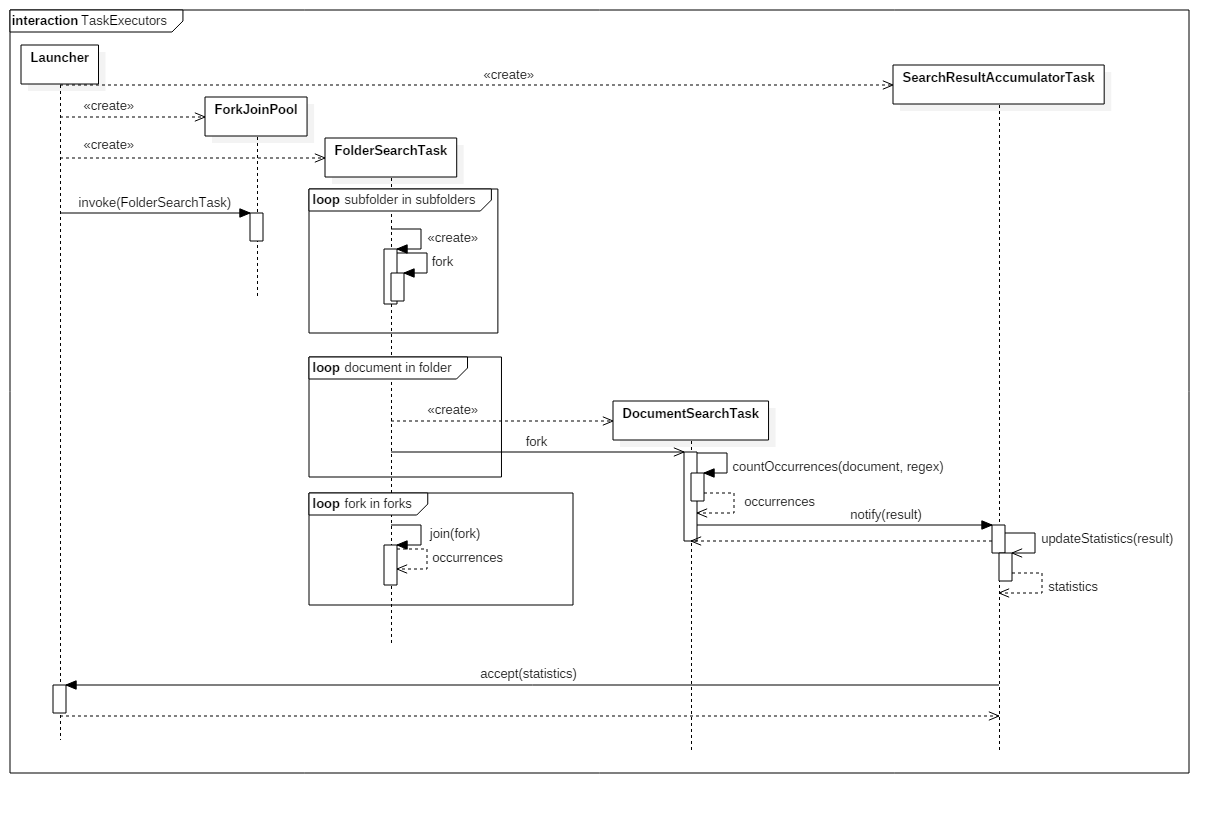
\includegraphics[width=\linewidth, height=\textheight,keepaspectratio]{TaskExecutors}

    \caption{Diagramma di sequenza dell'Esercizio 1}

    \label{fig:task-executors}

\end{figure}
\newpage
\subsubsection{Esercizio 2: Event Loop}

Come implementazione del modello a Event Loop \`e stato utilizzato il framework Vert.x \footnote{\url{https://vertx.io}}.

Analogamente all'Esercizio 1 il problema di partenza \`e stato scomposto in tre sottoproblemi, in questo caso risolti da tre tipologie di Verticle:

\begin{itemize}
%
    \item \texttt{FolderSearchVerticle}: ricerca delle occorrenze dell'espressione regolare in una cartella
%
    \item \texttt{DocumentSearchVertice}: ricerca delle occorrenze dell'espressione regolare in un documento
%
    \item \texttt{SearchResultAccumulatorVerticle}: aggregazione dei risultati e calcolo delle statistiche
%
    \item \texttt{SearchCoordinatorVerticle}: controllore del numero di documenti processati
%
\end{itemize}

Si \`e scelto di mantenere un numero fisso di istanze per ogni tipologia di Verticle.
%
Nel caso del \texttt{SearchResultAccumulatorVerticle} l'istanza \`e unica, mentre per le altre due tipologie di Verticle il numero di istanze pu\`o variare al fine di parallelizzare il carico di lavoro.

La comunicazione tra i Verticle si basa sullo scambio di messaggi attraverso un canale condiviso (Event Bus): ogni tipologia di Verticle ascolta su un canale dedicato.

Inizialmente viene mandato un messaggio al \texttt{SearchCoordinatorVerticle} con il numero totale di documenti da processare. 
%
La ricerca inizia inviando un messaggio contenente la radice dell'albero all'indirizzo dedicato alla ricerca all'interno di una cartella.
%
Il Verticle che riceve il messaggio (\texttt{FolderSearchVerticle}) visita tutte le sottocartelle e, per ognuna di esse, invia un messaggio allo stesso indirizzo.
%
In questo modo un altro \texttt{FolderSearchVerticle} provveder\`a alla ricerca nella sottocartella e cos\`i via.
%
Analogamente, per ogni documento, viene inviato un messaggio ad un \texttt{DocumentSearchVerticle} che provveder\`a alla ricerca delle occorrenze dell'espressione regolare fornita in input nel documento inviatogli.
%
Ogni \texttt{DocumentSearchVerticle}, dopo aver contato il numero di occorrenze, invia un messaggio con il risultato al \texttt{SearchResultAccumulatorVerticle}. Quest'ultimo, dopo aver aggiornato le statistche, chiama una callback responsabile di aggiornare l'output.
%
Infine il \texttt{DocumentSearchVerticle} invia un messaggio al \texttt{SearchCoordinatorVerticle} per comunicargli che l'analisi del documento in esame è terminata. Con questa informazione il coordinatore è in grado di capire quanti documenti devono essere ancora processati, così quando tutti i documenti sono stati controllati può informare il chiamante che il lavoro è concluso.
%

\begin{figure}[H]

    \centering

    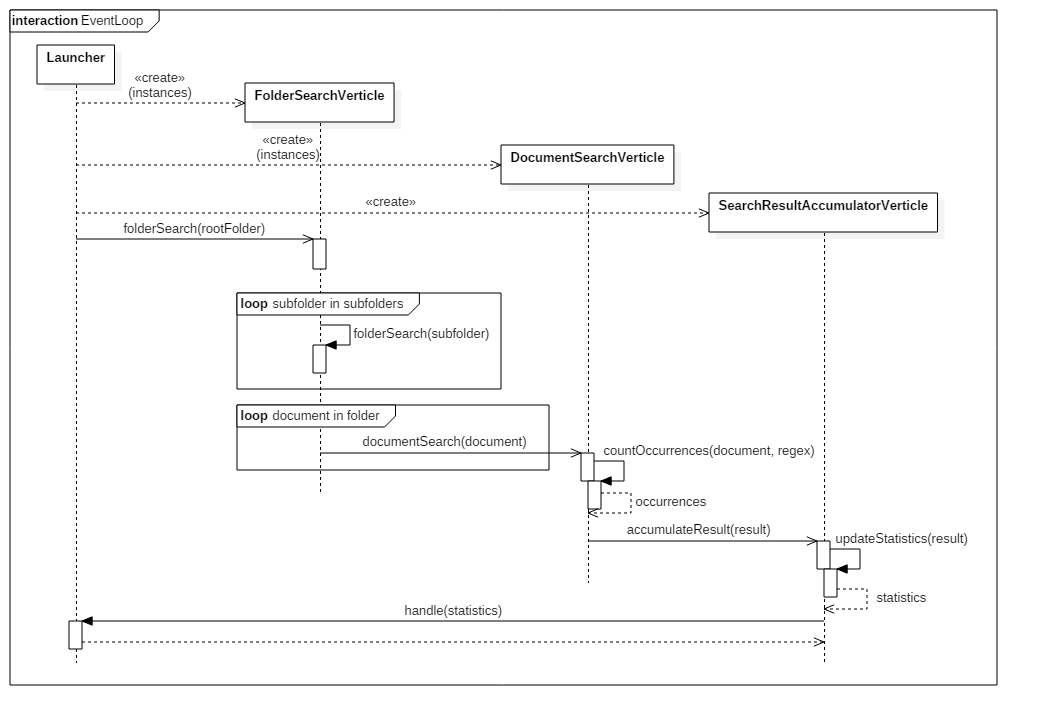
\includegraphics[width=\linewidth, height=\textheight,keepaspectratio]{EventLoop}

    \caption{Diagramma di sequenza dell'Esercizio 2}

    \label{fig:event-loop}

\end{figure}

\subsubsection{Esercizio 3: Reactive Streams}

Come implementazione dei flussi reattivi abbiamo utilizzato la libreria RxJava2 \footnote{\url{https://github.com/ReactiveX/RxJava}}.
%
L'approccio dichiarativo fornito dall'utilizzo dei Reactive Stream permette di semplificarne la soluzione.
%
In questo caso l'insieme di documenti \`e visto come flusso reattivo al quale \`e possibile applicare operazioni di trasformazione, di calcolo e di sottoscrizione.
%
Abbiamo scelto di utilizzare il costrutto \texttt{Flowable} perch\'e implementano i flussi reattivi \footnote{\url{http://www.reactive-streams.org}} ed il meccanismo di backpressure che permette di ottimizzare l'elaborazione dei flussi che emettono elementi ad una velocit\`a maggiore di quella con cui vengono elaborati.

Il flusso di dati \`e stato creato a partire dalla radice dell'albero di cartelle: cottenendo ricorsivamente i documenti di ogni cartella e sottocartella e trasformandoli in un unico flusso di documenti.
%
Generato il flusso specifichiamo su quale \texttt{Scheduler} verrano eseguite le manipolazioni.
%
Per ogni documento del flusso contiamo il numero di occorrenze dell'espressione regolare fornita in input e lo trasformiamo in un \texttt{SearchResult}.
%
A questo punto sottoscriviamo \texttt{SearchResultSubscriber} al flusso utilizzando il metodo \texttt{blockingSubscribe()}: questa scelta permette di sospenderci sul thread corrente finch\'e tutto il flusso non \`e stato processato, in caso contrario il thread corrente terminerebbe prima che tutti gli elementi emessi nell flusso reattivo siano processati.

\texttt{SearchResultSubscriber} implementa l'interfaccia \texttt{Subscriber}, permettendogli di sottoscriversi al flusso reattivo e di essere notificato quando il prossimo elemento \`e disponibile e quando il flusso \`e terminato.
%
All'arrivo di un nuovo elemento si occupa di aggiornare i risultati e della aggiornamento delle statistiche, che vengono passate ad una callback responsabile dell'aggiornamento dell'output.

\begin{figure}[H]

    \centering

    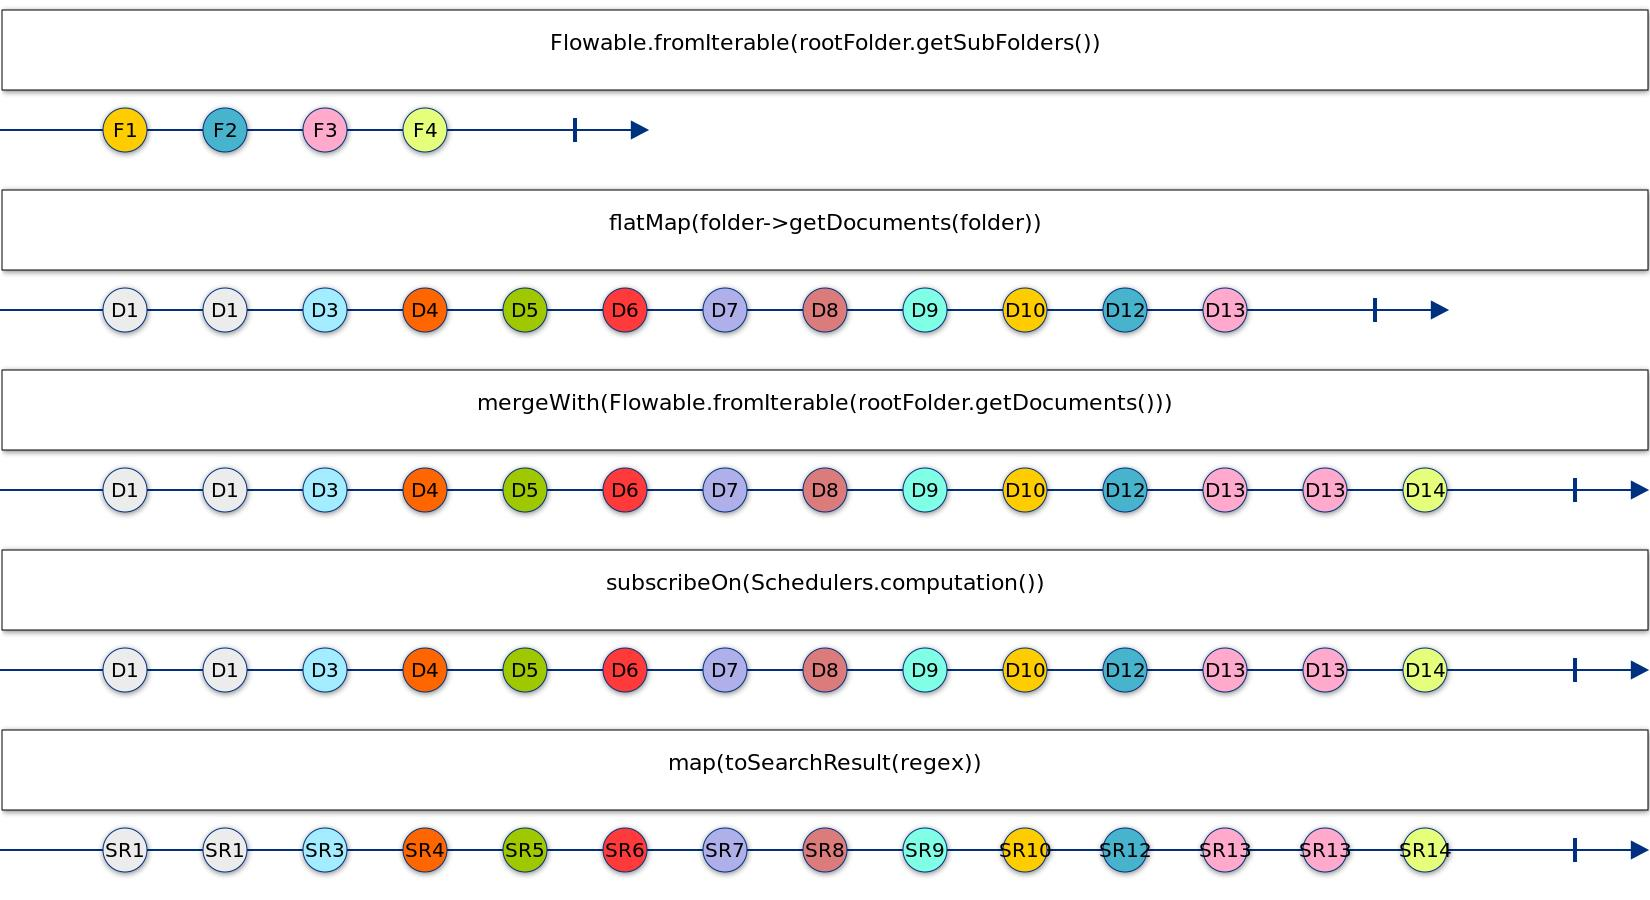
\includegraphics[width=\linewidth, height=\textheight,keepaspectratio]{ReactiveStreams}

    \caption{Marble Diagram dell'Esercizio 3}

    \label{fig:event-loop}

\end{figure}

\section{Analisi delle prestazioni}\label{analisi-delle-prestazioni}

Le prestazioni sono state valutate considerando i tempi di esecuzione di ogni esercizio.
%
Il calcolo delle statistiche \`e stato automatizzato tramite un apposita classe \texttt{Benchmark}.

\begin{table}[H]

\centering

\label{my-label}

\begin{tabular}{l|ccc}
\hline
    & Executors & Event Loop & Reactive Streams \\ \hline
Min & 23        & 23         & 26               \\
Max & 108       & 55         & 122               \\
Avg & 31        & 29         & 33               \\ \hline
\end{tabular}

\caption{Tempi aggregati di esecuzione delle tre soluzioni. I tempi sono espressi in millisecondi, considerando come percordo di partenza la radice del progetto, ricercando l'espressione regolare 'class' e specificando come profondità massima 25.
Le velocità di esecuzione sono state calcolate su un Apple Macbook Pro (Retina, 15", metà 2015) dotato di un processore Intel Core i7 quad-core a 2.2GHz.}

\label{Tabella speedup del sistema}

\end{table}

% Your document ends here!
\end{document}
